% !TeX root = ../main.tex

\chapter{Related work}  \label{chapter:relatedwork}

This chapter presents existing deep learning approaches that have addressed the issue of future frame prediction. These are grouped into three sections depending on the model implementation, namely neural networks, recurrent networks and adversarial networks. The strengths, weaknesses and design decisions of these models are briefly discussed together with a short analysis of the achieved outcomes. Further, it is highlighted how these approaches have influenced the architecture of our final model that is used throughout the evaluation in Chapter \ref{chapter:evaluation}. Aside from that, their results form the baseline in the assessment of our model.


\section{Neural Network Approach}

First approaches to predict future frames in an image sequence were made in \parencite{ann} and its follow-up publication \parencite{ann2}. Probably due to the lower computational power and the weak development of CNNs at that time, they tried to perform single frame prediction based on an artificial neural network. They performed several preprocessing steps in order to train such a model using image data. Firstly, the image data was partitioned by the R, G and B color channels into three parts. Next, the dimension of data was reduced from the order of $10^4$ to $100$ in each part using techniques like \textit{principle component analysis} (PCA)\footnote{PCA: Technique to reduce the data dimensionality by mapping it into its eigenspace.}. The final training and inference was then accomplished on three separate neural networks of the same architecture for each color channel. After each prediction, the PCA process was inverted to obtain the initial dimensionality, as well as all three outputs were combined to obtain the final image.

\begin{figure}[htb]
\centering
\begin{subfigure}{0.5\textwidth}
  \centering
  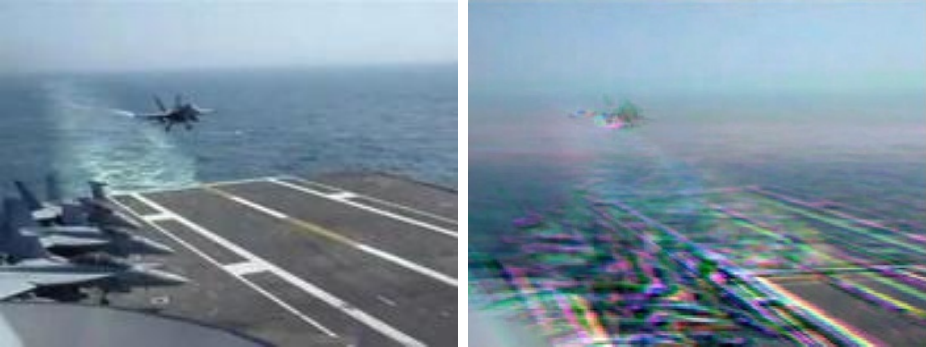
\includegraphics[height=2.1cm]{figures/related/fighter.png}
  \caption{Fighter dataset}
  \label{fig:aan_samples_fighter}
\end{subfigure}%
\begin{subfigure}{0.5\textwidth}
  \centering
  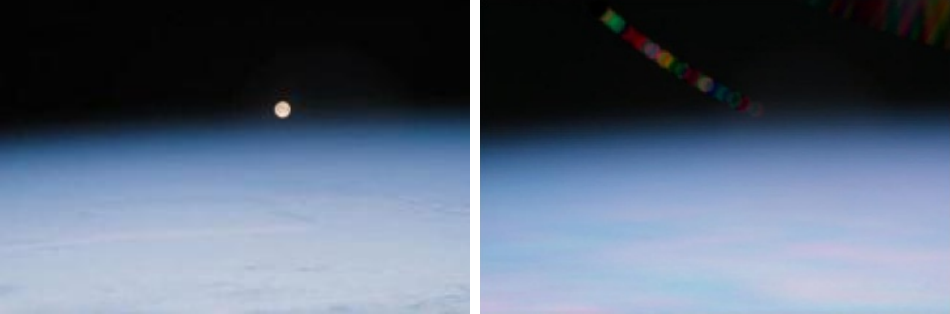
\includegraphics[height=2.1cm]{figures/related/nasa.png}
  \caption{NASA dataset}
  \label{fig:aan_samples_nasa}
\end{subfigure}
\caption[ANN Frame Prediction]{Single frame predictions using an ANN model with two hidden layers.\\
Left: ground truth target frame. Right: generated prediction. (From \parencite{ann})}
\label{fig:aan_samples}
\end{figure}

The loss during the training process is measured in terms of the MS-SSIM index in order to optimize the network to preserve the luminance, contrast and structure of the image. Since the data of the used Fighter and NASA datasets have a high image size, applying the multi-scale version of SSIM is a reasonable choice.

When we take a look at the presented prediction results in Figure \ref{fig:aan_samples}, it can be seen that the network more or less averages over the input sequence. This effect is clearly visible in Figure \ref{fig:aan_samples_nasa}, where the movement of the moon from the top left towards the earth's horizon is predicted like being composed of previous moon positions. As a result, this simple architecture does not sufficiently capture the temporal correlations of the input data.

\section{Recurrent Network Approaches}

In order to leverage the sequential structure and temporal correlations of video data, several works performed frame prediction based on recurrent network models. The following models have inspired our final model architecture the most.

\subsection{LSTM Encoder-Decoder-Predictor Model}

A huge step forward was made when the recurrent encoder-decoder framework, earlier presented in Section \ref{sec:rnn_enc_dec}, was applied in \parencite{unsup_learn_lstm} to perform unsupervised learning of video representations. The fact that the same operation should be applied at each time step to produce the next state was their key idea to use this framework in that context. 

All in all, they preseted a LSTM autoencoder model that is trained to reconstruct an entire input sequence of about ten image frames, similar to Figure \ref{fig:rnn-autoencoder}. This model was then slightly modified in a second step to predict the future sequence of frames. In a last step, both models were combined to a single model that contains only one encoder to learn the dynamics of the video, but two separate encoder networks. Initialized by a copy of the learned representation, one decoder tries to reconstruct the inputs backward in time, while the other decoder predicts the future frames forward in time. Consequently, the decoder has to come up with a representation that can be handled by both decoders. In this way, they tried to compensate the shortcomings of each model, such as the potential tendency of the reconstruction decoder to learn the trivial function, or to counteract that the future predictor considers the last frames of the input sequence only. This combined model delivers the best results and is shown in Figure \ref{fig:lstm_combo}.

\begin{figure}[htb]
	\centering
	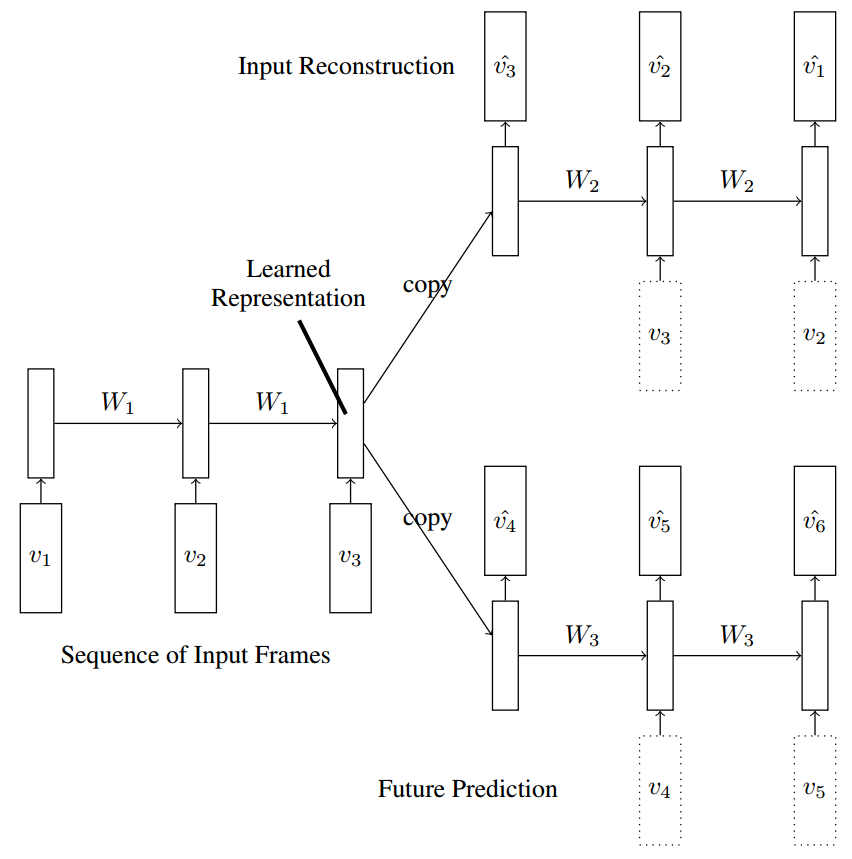
\includegraphics[width=0.5\linewidth]{figures/related/combo_shrinked.png} 
	\caption[Composite LSTM Autoencoder Model]{The composite LSTM autoencoder model. The top branch reconstructs the input sequence backwards in time, while the bottom branch performs frame predictions forward in time. (From \parencite{unsup_learn_lstm})} \label{fig:lstm_combo}
\end{figure}

Within their work, they also explored if the decoder should condition on the previously generated output or not, as earlier discussed in Section \ref{sec:rnn_enc_dec}. The final choice has fallen on the conditioned variant because it delivered slightly sharper frame prediction results in the qualitative evaluation. Besides that, they also varied the number of recurrent layers with the clear result that deeper LSTMs yields best performance.

Another contribution of this work was the introduction of a simple dataset that can be generated on-the-fly in order to explore the architecture of the model, as well as the effects of hyperparameter changes. It uses handwritten numbers that bounce around in a short sequence of images. Since this dataset is used in several other subsequent works as well, it offers the ability to be used as a basic benchmark to compare the performance of various models. The dataset is presented later in Section \ref{sec:ds_mm}. Sequences from this and another dataset were then used as input to the LSTM encoder to train the model. It must be highlight that they utilize the full image patch for this purpose. They have also mentioned to use convolutional percepts of the image sequence as inputs, but actually used this approach in the second part of their paper only, where the pre-trained encoder was transferred to improve the performance of supervised human action classification in videos.

The authors also pointed out that the choice of the loss function is fundamental with respect to the quality of results. Nevertheless, they decided to rely on standard error functions and kept the use of more advanced objective functions for further research. To be more precise, they trained their network using binary cross-entropy when being applied to Moving MNIST, and squared error for real world tests on UCF-101. Details about the latter dataset can be found in Section \ref{sec:ds_ucf}.

All in all, the strength of this model regarding future frame prediction is that it is able to infer a variable number of frames by taking the temporal correlations of the entire input sequence into account. But as a downside, the use of FC-LSTM cells with such high dimensional inputs implies a huge model complexity in the order of $10^8$ in case of a two-layer LSTM with \num{2048} hidden units each. Consequently, such a model takes a very long time to learn useful patterns. Furthermore, it does not consider spatial properties of each single input due to the use of fully-connected state transitions.


\subsection{Convolutional LSTM Encoding-Forecasting Model} \label{sec:related-convlstm}

The previously described model was extended in \parencite{conv_lstm_nowcasting} with the general goal to develop a deep learning approach for precipitation nowcasting\footnote{Precipitation nowcasting: short-term forecasting of rainfall.}. But in order to moderate the tremendous redundancy of spatial correlations in standard FC-LSTM cells, they invented a modified version of LSTM that features convolutional structure for both input-to-state and state-to-state transitions. More details regarding its formulation and internal structure follows in Section \ref{sec:conv_lstm}. To put it in a nutshell, they exchanged each matrix multiplication by a convolution operation whereby the internal states become three dimensional tensors\footnote{Tensor: multidimensional data array that flows through the computation graph. It's shape can change when passing any neural network layer.} and preserve spatial information. These \textit{convolutional LSTM} (ConvLSTM) cells are then used in the same decoder-encoder framework as before, like illustrated in Figure \ref{fig:convlstm_model}. At the bottom line, these cells are able to capture spatio-temporal properties of the data much better than FC-LSTM cells and have shown to outperform them with even containing way less model parameters.

\begin{figure}[htb]
	\centering
	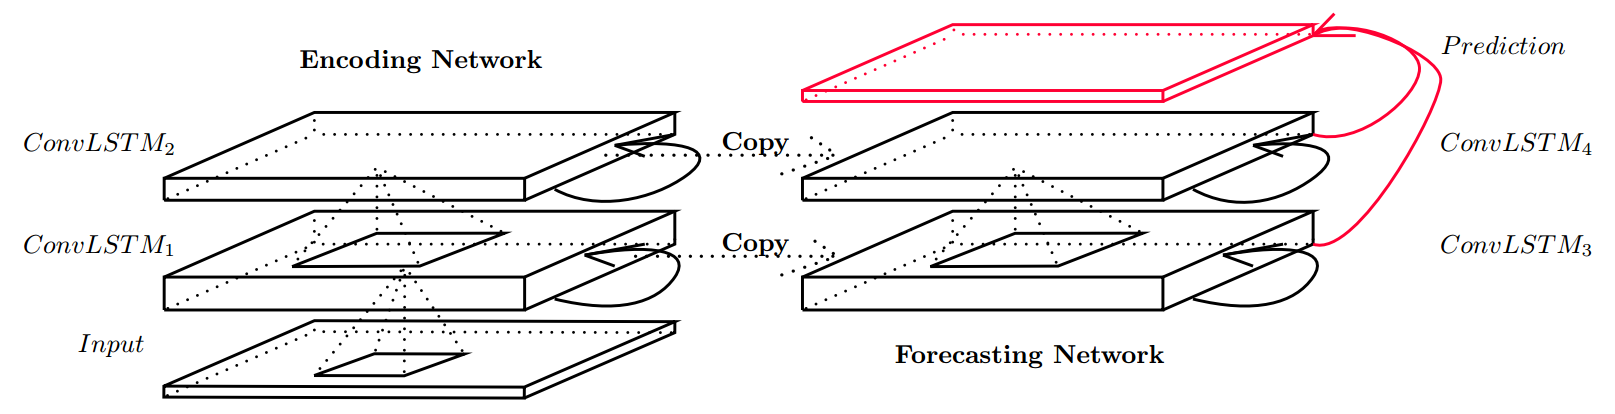
\includegraphics[width=0.8\linewidth]{figures/related/nowcasting_model.png} 
	\caption[ConvLSTM Encoding-Forecasting Model]{The ConvLSTM encoding-forecasting model that was used in the paper in context of frame prediction and precipitation nowcasting. (From \parencite{conv_lstm_nowcasting})} \label{fig:convlstm_model}
\end{figure}

Among other datasets, the authors trained this model on Moving MNIST in the course of their work and therefore it is another good candidate to compare our model with. The model was thereby fed with reshaped tensors of size $16 \times 16 \times 16$ by splitting the original frames using a $4 \times 4$ grid \parencite[p. 6]{conv_lstm_nowcasting}. The reason for this reshaping was not argued in the paper, despite the fact that this unnecessarily increases the spatial redundancies. But since it divides the size of the image by a factor of 16, one simple reason might be to reduce the computational complexity because the depth is increased by the ConvLSTM's convolutions nevertheless. To generate the final prediction, the state of each ConvLSTM layer per time step $\tau$ is concatenated and fed into a $1 \times 1$ convolutional layer for the purpose of reducing their depth to match with the ground truth target \parencite[p. 4]{conv_lstm_nowcasting}. Also at this point, it was not explained why the concatenated hidden state of all layers is used to generate the prediction, instead of the more intuitive choice of only relying on the the final layer'w output.

To condense the three most important findings of their evaluations, it was shown that the kernel size of the state-to-state transitions has to be at least bigger than $1 \times 1$ to capture spatio-temporal motion patterns. The windows size of this kernel can be interpreted as the maximum motion that the model is able to detect from one time step to the next. The second outcome is that deeper models can produce better results even when each layer contains fewer parameters. And last but not least, as already stated earlier in this section, the use of convolutional LSTM cells instead of FC-LSTM cells enables to reach better performance with less training examples, requires less iterations to converge and is less likely to overfit.


\subsection{Spatio-Temporal Video Autoencoder Model}

A second work using ConvLSTM cells was published in \parencite{spat_temp_video_autoenc}. It is based on the fundamental idea that a video autoencoder should differ from spatial autoencoders by being able to encode the significant differences instead of memorizing the entire video sequence. With such an encoding at hand, neural networks should be able to learn the generation process of the future for any given frame. Compared to both previous models, this one does not rely on the standard recurrent decoder-encoder framework. Instead, it uses convolutional layers followed by a ConvLSTM encoder to produce a dense transformation map as its learned representation. Afterwards, a semi-detached optical flow module serves as a temporal decoder on the basis of the learned transformation map. The estimated optical flow is then applied to the current image in order to generate the next frame using a convolutional decoder. This architecture is demonstrated in Figure \ref{fig:spatiotemp_model}.

\begin{figure}[htb]
	\centering
	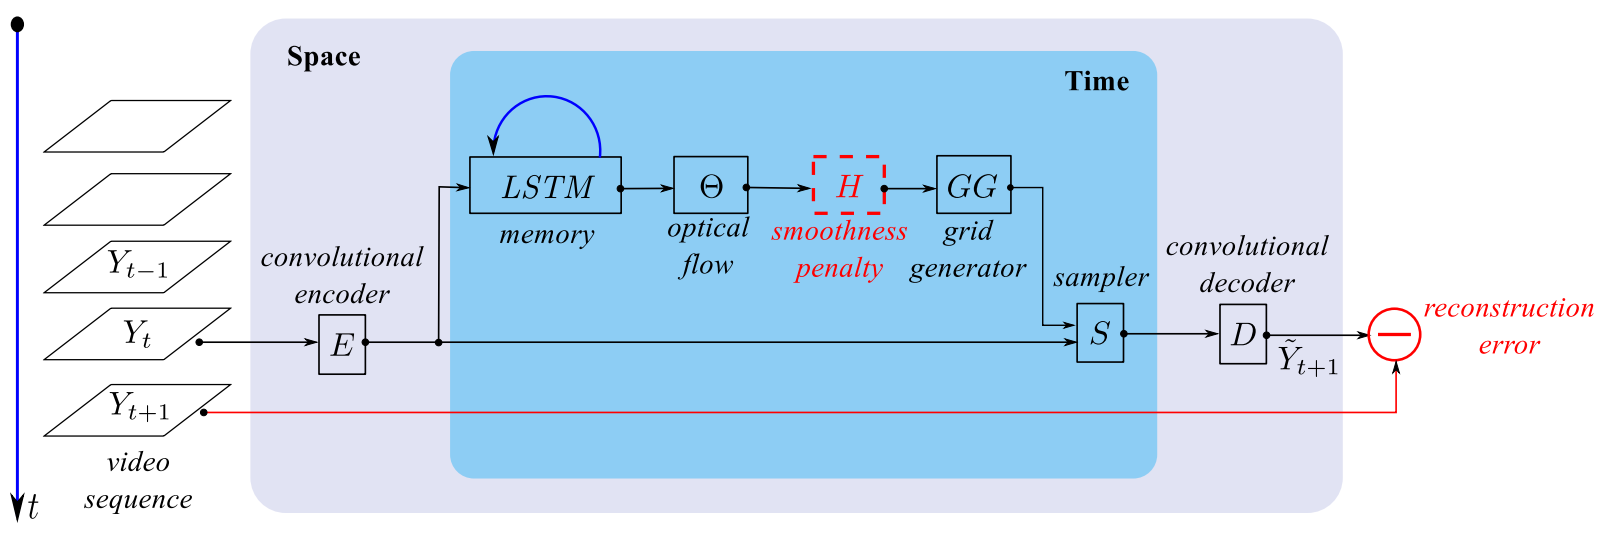
\includegraphics[width=0.9\linewidth]{figures/related/spat_temp_video.png} 
	\caption[Spatio-Temporal Video Autoencoder Model]{The spatio-temporal video autoencoder model with its components that are separated by the space and time domain. (From \parencite{spat_temp_video_autoenc})} \label{fig:spatiotemp_model}
\end{figure}

The vanilla version\footnote{Vanilla version: an often used term in deep learning that refers to the standard configuration of something.} of the described model uses a single convolutional layer in the spatial encoder or decoder with \num{32} filters and a kernel of size $7 \times 7$ each. The temporal encoder comes with the same kernel size, but \num{45} filters from one time step to the next. This model exhibits a total number of only \num{703651} model parameters. 

For the assessment of the model, they used the Moving MNIST dataset as well, but unfortunately in context of single frame prediction only. The binary cross-entropy cost function in combination with binary MNIST data was used in the first as well, but also other loss functions for floating-point MNIST data like $\ell_2$, a variant of gradient difference loss, as well as the sum of both. The latter combined loss has thereby achieved the best qualitative and quantitative results in the final analysis. Some sample results from their paper are depicted in Figure \ref{fig:spatiotemp_results}, including comparisons to other architectures of previously presented models. Besides that, various depth combinations of each encoder or decoder component were evaluated as well. They ended up with the final result that deeper models clearly achieve better performance, regardless of whether it is about the space or time domain.

\begin{figure}[htb]
	\centering
	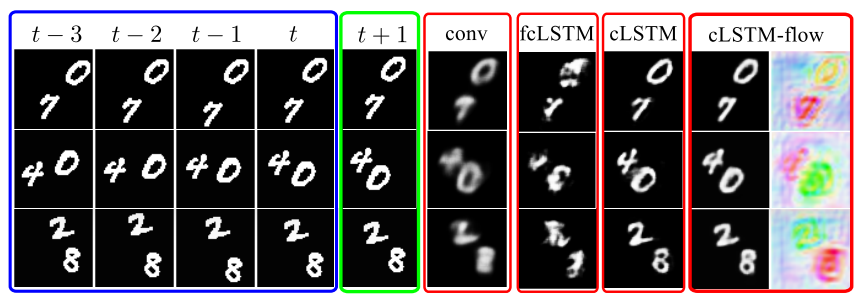
\includegraphics[width=1.0\linewidth]{figures/related/spat_temp_results.png} 
	\caption[Qualitative Moving MNIST Results of LSTM Models]{Qualitative comparison of results on MovingMNIST using different model architectures. Blue: the last 4 out of 10 frames fed into the network. Green: the next frame's ground truth. Red: Prediction results on various models in comparison, where \textit{conv} is a simple convolutional autoencoder that handles each frame as a separate input channel, and \textit{cLSTM-flow} is the model presented in this section. (From \parencite{spat_temp_video_autoenc})} \label{fig:spatiotemp_results}
\end{figure}

A possible downside of this model is the fact that is was trained to predict one single frame only. Even though the predicted results in Figure \ref{fig:spatiotemp_results} look very similar to its ground truth future, it was not shown how the performance continues over the course of the following predictions in the future. One may assume that because each single predicted frame is slightly blurry compared to images from the input sequence, it might happen that the prediction quality of further frames could decrease rapidly. As a matter of fact, the model has never seen any blurry image example during the whole training process. At least such a fast decrease in quality was experiencedd during the development of the final architecture, after starting with a simple convolutional encoder-decoder model that produced a single frame only, together with a sliding window approach to produce the following future frames.

On the opposite side, this work offers several interesting insights to learn from as well. For one thing, it emphasizes the power of ConvLSTM cells regarding spatio-temporal learning once more, for another thing, it has shown that the use of convolutional percepts as input to the recurrent encoder offers another possibility to improve the results. The latter also reduces the dimensionality that has to be processed by condensing the input data. The final model architecture, that is presented in Chapter \ref{chapter:implementation}, takes advantage from both of them.


\section{Adversarial Network Approach} \label{sec:related_gan}

In the final stage of this thesis, we came across a novel approach to train neural networks to perform frame prediction without using recurrent cells. The authors of \parencite{deep_multiscale_video_pred} used a very simple, overcomplete convolutional generator network $ G(X) $ in order to generate a single or multiple frames from an input sequence $ X $. This simple network is displayed in Figure \ref{fig:gan_generator} and consists of only convolutional layers, with a constant height and width but variable number of feature maps. Training a model of such a simple architecture has several weaknesses, such as that it could only capture short-range dependencies across the entire input sequence with the size of the kernel, due to the fixed size feature maps. Also, default loss functions such as $\ell_1$ or $\ell_2$ during the training experientially lead to blurry results, as previous studies have already shown.

\begin{figure}[htb]
	\centering
	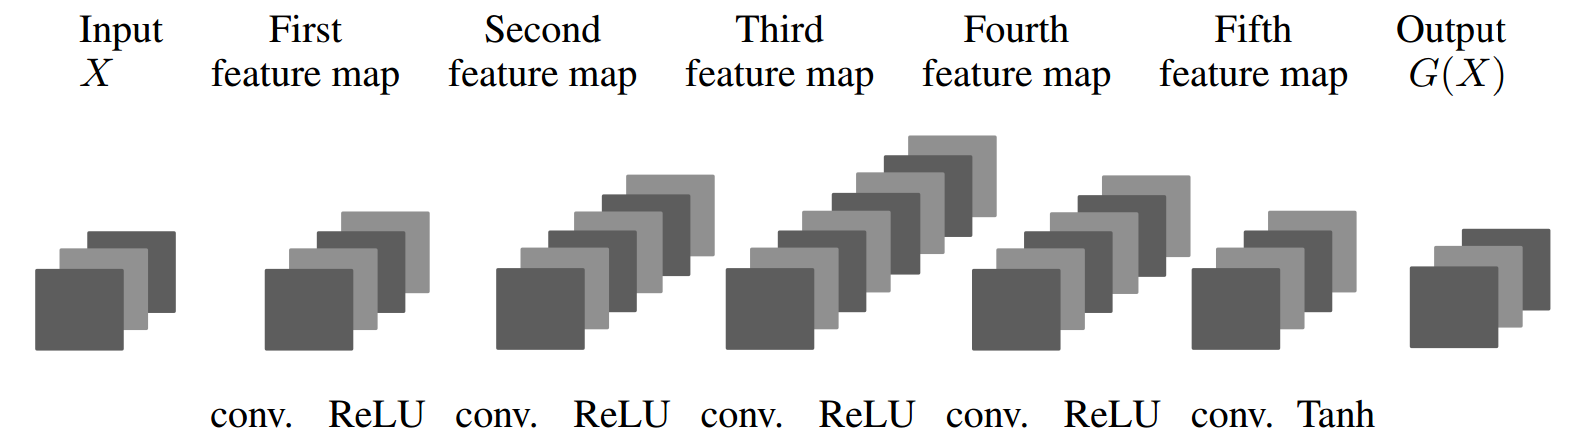
\includegraphics[width=0.8\linewidth]{figures/related/deep_multiscale_generator.png} 
	\caption[Convolutional Autoencoder for Future Generation]{A very basic convolutional network that maps a fixed number of input frames $X$ to predict one or multiple future frames $\hat{Y} = G(X)$. The feature maps exhibit the same height and width at each layer, but different depths. (From \parencite{deep_multiscale_video_pred})} \label{fig:gan_generator}
\end{figure}

To overcome these issues, they proposed three different but complementary learning strategies. Firstly, they used a multi-scale approach where multiple generator networks are iteratively trained on different scales of the input patch, starting from the lowest scale. The prediction of the next larger scale then used the upscaled prediction of the previous scale as a starting point. This technique enabled the network to consider motion patterns of longer range\footnote{It is to add that networks using ConvLSTM cells do not suffer from the issue of being limited to short-range dependencies in such an extend, because the used state-to-state kernel size determines the maximum motion from one time step to the next. In contrast, the kernel size of this convolutional autoencoder defines the maximum motion across the entire input sequence. Thus, a multi-scale approach is not necessarily required for networks using ConvLSTMs for this purpose.}. Secondly, they extended their loss function with an additional GDL term in order to penalize blurry outputs in image space. This gradient-based loss function has already been introduced in Section \ref{sec:gdl}. And lastly, they plugged this simple convolutional network into the adversarial training framework. The described network therefore defines a generator network $G$ to predict the next frame, while a second discriminator network $D$ is consulted in order to assess whether the output of the generator network is the real target frame of the future or just a generated fake. Using an alternating training procedure, both networks learn to perfect the system. In other words, the discriminator network of this adversarial training process can be seen as an adaptive loss layer that assesses the generated output in feature space. Also other works highlight the usefulness of considering the error in feature space in addition to the image space error, such as in \parencite{gen_img_perc_sim}. Summarizing the last two proposed learning strategies, a triplet loss is used where a standard loss function in image space in combined with a perceptional motivated loss function to preserve sharpness, as well as an adversarial error function which quantifies the realness of the generated frames. 

\begin{figure}[htb]
	\centering
	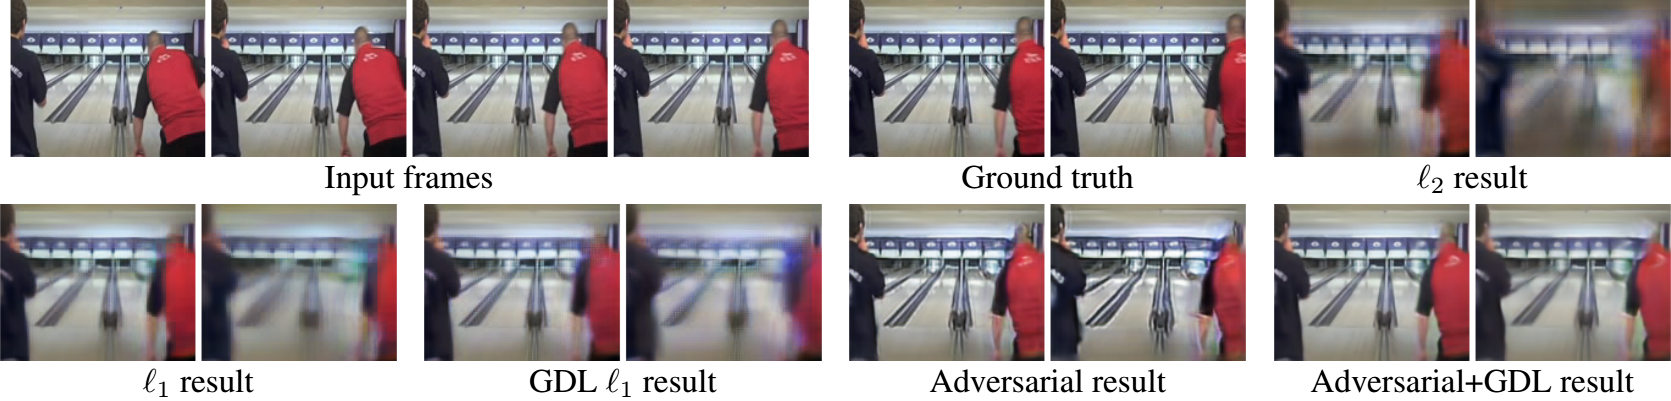
\includegraphics[width=1.0\linewidth]{figures/related/deep_multiscale_samples.png} 
	\caption[Comparion of Loss Functions in GAN Model]{Comparison of different loss function combinations using a simple CNN to predict one frames given four inputs. The second future frame is predicted recursively. (From \parencite{deep_multiscale_video_pred})} \label{fig:gan_samples}
\end{figure}

The performance of different loss function combinations was also compared in a qualitative evaluation. Several output samples are shown in Figure \ref{fig:gan_samples}. As can be seen, the combination of multiple loss functions with different objectives enables to end up with predictions of higher quality and realism. Besides that, a detailed comparison to other LSTM based models on the UCF-101 video dataset was given. Thus, it allows us to compare our outcomes to all these results as well.

But even when this network using all the proposed learning strategies is able to produce outstanding frame prediction results, it comes with some weaknesses nevertheless. For instance, the temporal correlations of the input sequence are not explicitly modelled in the generator network. Hence, it has to explore the sequential structure of the data by its own from scratch. Furthermore, adversarial networks are said to be hard to train, because the oscillating loss values of the generator and discriminator networks are tough to interpret. Also, experience is of advantage, since the learning rates of both networks have to be kept in balance.
